%%%%%%%%%%%%%%%%%%%%%%%%%%%%%%%%%%%%%%%%%%%%%%%%%%%%%%%%%%%%%%%%%%%%%%%%%%


% abnTeX2: Modelo de Trabalho Acadêmico em conformidade com 
% as normas da ABNT


%%%%%%%%%%%%%%%%%%%%%%%%%%%%%%%%%%%%%%%%%%%%%%%%%%%%%%%%%%%%%%%%%%%%%%%%%%


\documentclass[english, 
               brazil, 
               bsc] %Opções bsc (TCC) e msc (Mestrado)
               {dcomp-abntex2}




%%%%%%%%%%%%%%%%%%%%%%%%%%%%%%%%%%%%%%%%%%%%%%%%%%%%%%%%%%%%%%%%%%%%%%%%%%
% Área para adição de pacotes extras
%%%%%%%%%%%%%%%%%%%%%%%%%%%%%%%%%%%%%%%%%%%%%%%%%%%%%%%%%%%%%%%%%%%%%%%%%%


% \usepackage{lipsum} % Retirar para a versão final do documento
\usepackage{float}
\usepackage{pgfgantt}
\usepackage{lscape}


\restylefloat{table}


%Utilize aqui seu pacote preferido para algoritmos
\usepackage[linesnumbered]{algorithm2e}


%%%%%%%%%%%%%%%%%%%%%%%%%%%%%%%%%%%%%%%%%%%%%%%%%%%%%%%%%%%%%%%%%%%%%%%%%%


%Compila o índice
\makeindex


\begin{document}


% Seleciona o idioma do documento (conforme pacotes do babel)
\selectlanguage{brazil}


% Retira espaço extra obsoleto entre as frases.
\frenchspacing 


%%%%%%%%%%%%%%%%%%%%%%%%%%%%%%%%%%%%%%%%%%%%%%%%%%%%%%%%%%%%%%%%%%%%%%%%%%
% ELEMENTOS PRÉ-TEXTUAIS
%%%%%%%%%%%%%%%%%%%%%%%%%%%%%%%%%%%%%%%%%%%%%%%%%%%%%%%%%%%%%%%%%%%%%%%%%%


\pretextual




\titulo{PreOCR - Trabalho de Processamento de Imagens T01 2023.2} 
\autor{Grupo 13 - Everton Santos de Andrade Júnior}
\orientador{}
\coorientador{}


% \inserirInformacoesPDF





% \inserirInformacoesPDF
%
%
\imprimircapa
% \imprimirfolhaderosto*
%  
%     
\mostrarSUMARIO


%%%%%%%%%%%%%%%%%%%%%%%%%%%%%%%%%%%%%%%%%%%%%%%%%%%%%%%%%%%%%%%%%%%%%%%%%%
% ELEMENTOS TEXTUAIS
%%%%%%%%%%%%%%%%%%%%%%%%%%%%%%%%%%%%%%%%%%%%%%%%%%%%%%%%%%%%%%%%%%%%%%%%%%


\textual


%%%%%%%%%%%%%%%%%%%%%%%%%%%%%%%%%%%%%%%%%%%%%%%%%%%%%%%%%%%%%%%%%%%%%%%%%%
% Introdução
%%%%%%%%%%%%%%%%%%%%%%%%%%%%%%%%%%%%%%%%%%%%%%%%%%%%%%%%%%%%%%%%%%%%%%%%%%
\chapter{Introdução e Resultados} \label{introduction}

Neste trabalho, desenvolvemos um programa capaz de processar imagens binárias no formato PBM ASCII (PGM tipo P1), contendo texto dos tipos e tamanhos de fontes, variando de 10 à 40. Conseguimos determinar o básico do trabalho que são o número de linhas e palavras no texto e os retangulos dessas palavras, gerando uma imagem de saída com esses retangulos. Além disso, nosso grupo implementou mais funcionalidades, como a detecção de colunas e blocos do texto, utilizando o conceito de distância alinhada. Includingo a \textit{bouding box} (bbox) desses blocos e linhas que indicam as colunas.

Adicionalmente, para ilustrar nossos resultados de forma mais interativa, geramos uma série de imagens intermediárias que mostram o processo de detecção de blocos, colunas, palavras, e linhas destacando as regiões por um retangulo de diferentes cores. O formato dessas imagems é P3 (ascii RGB).
Essas imagens foram usadas em sequencia de frames para gerar um video de saíoda usando o programa de linha de commando ``ffmpeg``.

A nossa abordagem é dinamica, baseado na altura das palavras mudamos os parametros enquanto o programa roda. Desse modo é possivel identificar estruturas de texto em diferentes alinhamentos, como justificado, esquerda, centro e direita, além de lidar com diferentes tamanhos e estilos de fonte, incluindo Comic Sans, Impact, Cascadia Code, Arial e Times New Roman. Um exemplo de video gerado pode ser encontrado em \url{https://youtu.be/uA45GeodGss?si=ZOgsA2av7EKZeG69}.

Na \autoref{timesnewroman}
\begin{figure}[h]
        \caption{\label{timesnewroman} \small Times New Roman em itálico, com 4 colunas, 6 blocos de texto.}
        \begin{center}
            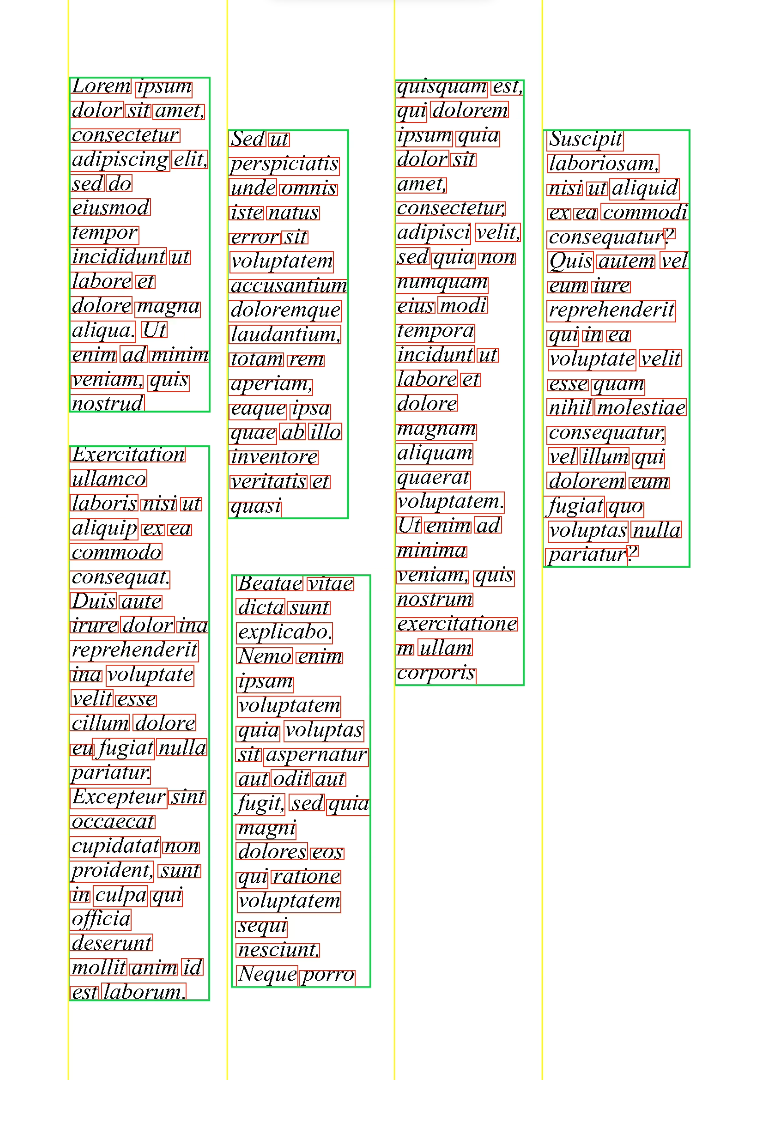
\includegraphics[scale=0.5]{./images/times_new_roman_italic_columns.png}
        \end{center}
  \legend{ \small Fonte: Autor.}
\end{figure}

\begin{figure}[h]
        \caption{\label{cascadia} \small Cacadia Code em negrito com tamanho 10, 2 colunas e 5 blocos de texto. A entrada possue baixa resolução e ruídos. }
        \begin{center}
            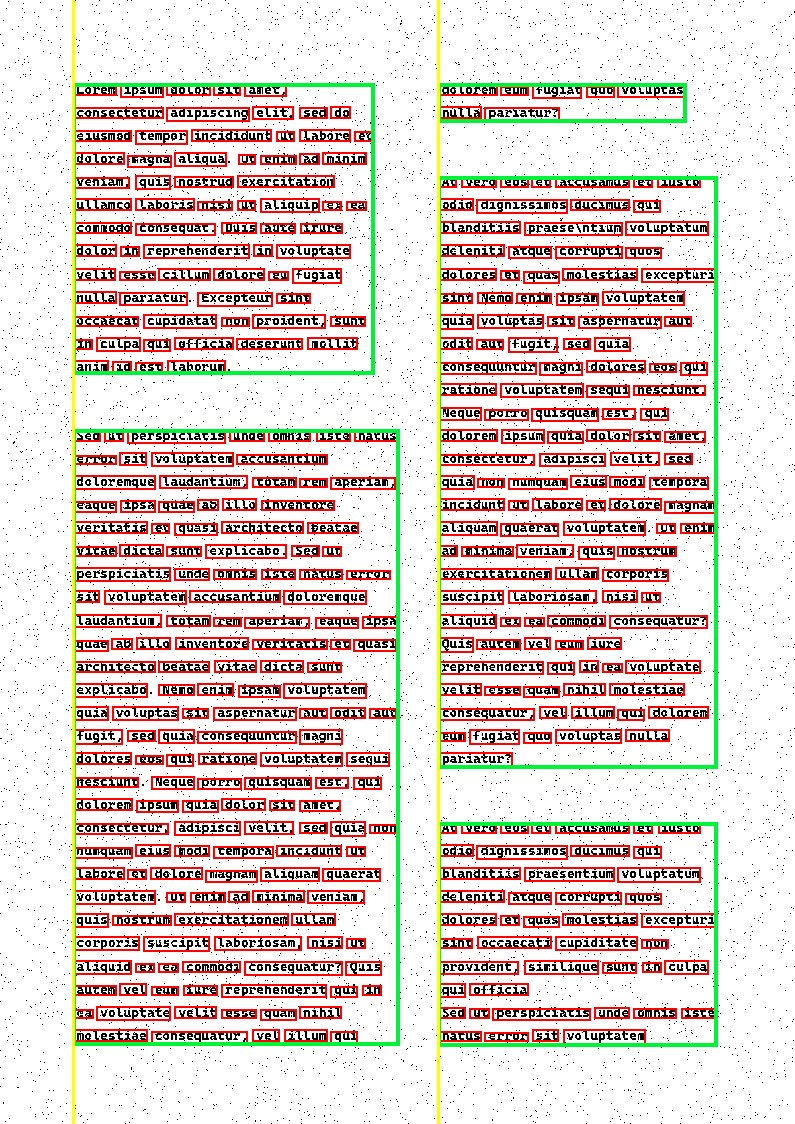
\includegraphics[scale=0.5]{./images/cascadia_code_10_detected_colunas_2_blocos_5_linhas_42_palavras_395.png}
        \end{center}
  \legend{ \small Fonte: Autor.}
\end{figure}



\section{Resultados}

Inicialmente, o algoritmo lê a imagem de entrada e a pré-processa aplicando filtro da medianos (nome da função é no código \texttt{median\_blur}) e invertendo as cores. Essas etapas visam retirar possíveis ruídos do tipo sal de pimenta. O tamanho do filtro mediano é 3 de altura e largulo já que foi confirmado que os ruídos não passam do tamanho de 1 pixel. A inversão da imagem é feita para aplicar algoritmos morfológicos, como a dilatação, para melhorar a conectividade dos componentes de texto e facilitar o processamento subsequente. Dependendo dos parâmetros especificados, o algoritmo pode aplicar operações adicionais como fechamento (closing) ou abertura (opening) para refinar ainda mais as regiões de texto. A ideia é utilizar um elemento estruturante, conhecido como SE (do inglês, \textit{Structuring Element}), que connecte as letras; isso pode ser feito com um SE que seja horizontal. Foi testado com diferentes SEs, como fomarto circular, de cruz, vertical, mas o melhor é o horizontal. E faz sentido pois as letras vem logo à direta da anterior, então para conectalas, precisamos esticar na horizontal para "grudar" uma na outra. Veja como é da uma "esticada" para horzinhotal ao aplicar um SE [000] [111] [000].
\[
\begin{matrix}
0 & 0 & 0 \\
1 & 1 & 1 \\
0 & 0 & 0 \\
\end{matrix}
\]

Na \autoref{timesnewroman}
\begin{figure}[h]
        \caption{\label{timesnewroman} \small Times New Roman em itálico, com 4 colunas, 6 blocos de texto.}
        \begin{center}
            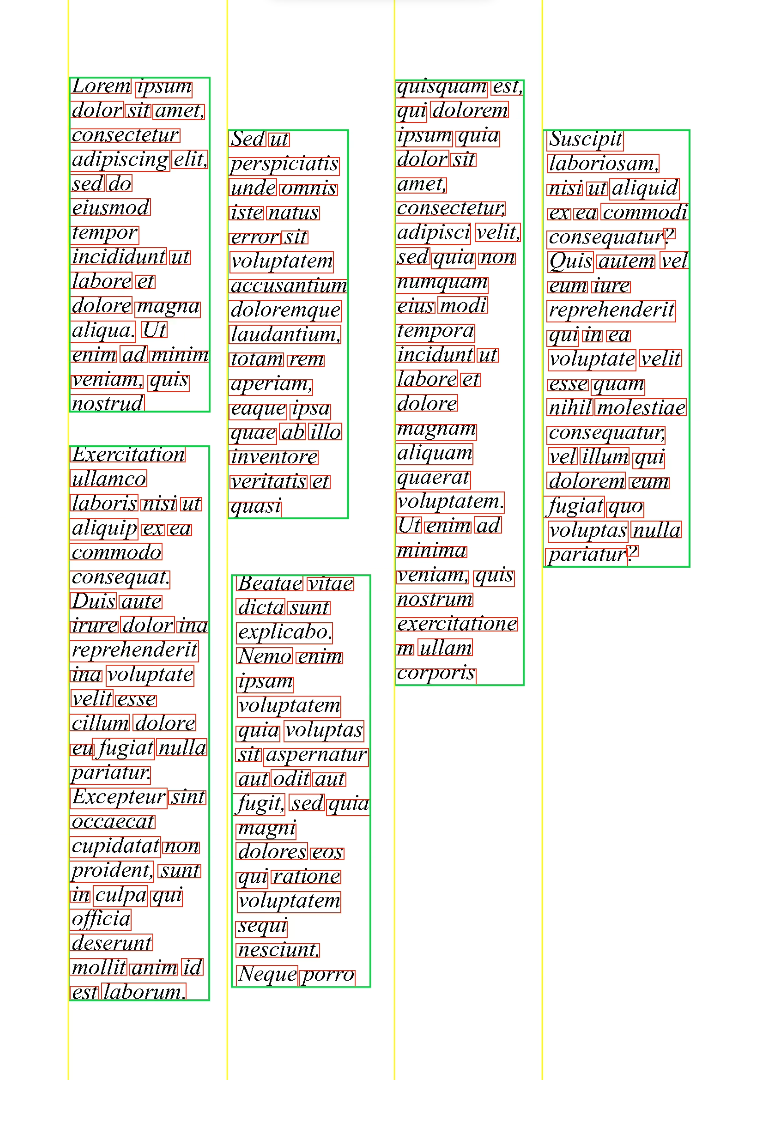
\includegraphics[scale=0.5]{./images/times_new_roman_italic_columns.png}
        \end{center}
  \legend{ \small Fonte: Autor.}
\end{figure}

\begin{figure}[h]
        \caption{\label{cascadia} \small Cacadia Code em negrito com tamanho 10, 2 colunas e 5 blocos de texto. A entrada possue baixa resolução e ruídos. }
        \begin{center}
            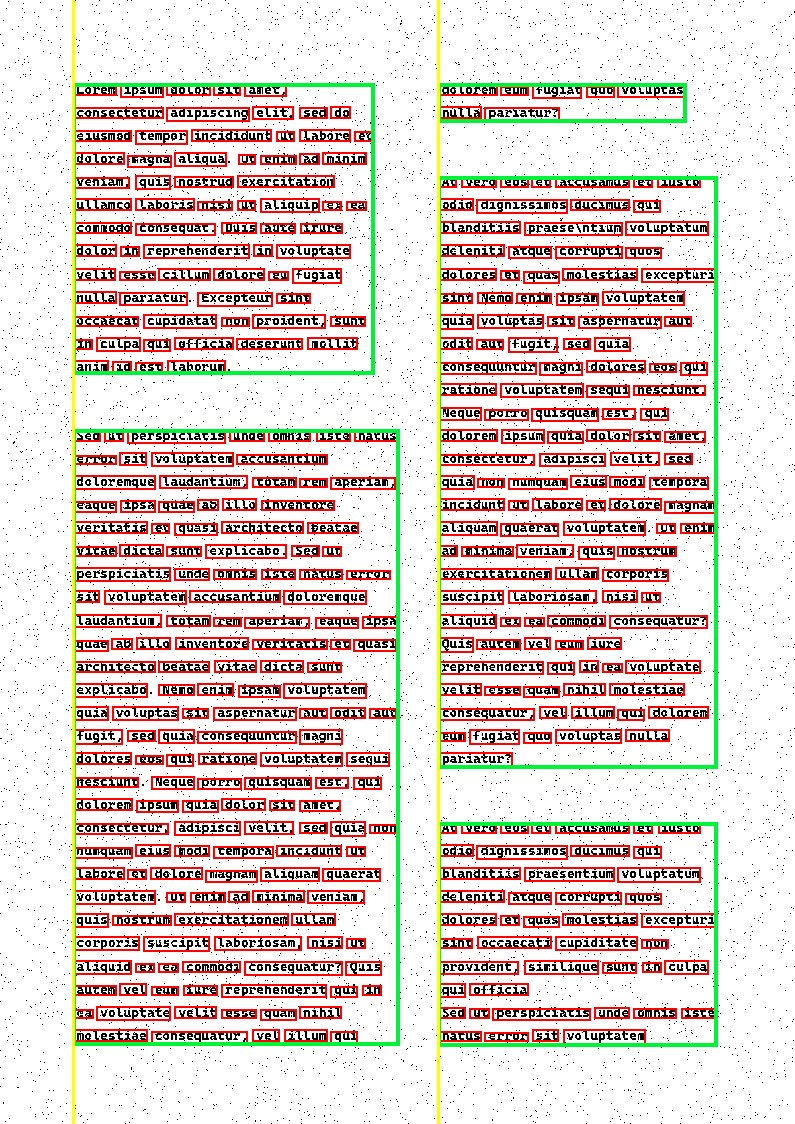
\includegraphics[scale=0.5]{./images/cascadia_code_10_detected_colunas_2_blocos_5_linhas_42_palavras_395.png}
        \end{center}
  \legend{ \small Fonte: Autor.}
\end{figure}


Aplicação de operações de dilatação horizontal para melhorar a conectividade entre caracteres adjacentes.
Após as operações morfológicas, indetificamos as palavras individuais através componentes conectados dentro da imagem. Cada palavra é contida em uma bbox, que é desenhada retângulos ao redor delas na imagem de saída. Componentes conectados  é um conceito de grafos que pode ser aplicado numa imagem binarias, pixels brancos são nós. Existem tipos de connectividade. Se consideramos os vizinhos de um pixel como apenas esquerda, direita, cima e baixo, então temos 4-conectividade \cite[2.5.2 Adjacency, Connectivity, Regions, and Boundaries]{gonzalez2008digital}. Se adicionarmos as diagonais, agora temos 8-conectividade. O Algortimo para encontrar esses componentes conectados se basea numa busca profunda, marcado os visitados, toda vez que na imagem for não zero fazemos a busca até não encontrar mais caminhos, considerando as digonais. Se não encontramos mais caminhos quer dizer que esse é um compoenente. Repetimos até encontrar todos atualizando o ponto mais a em esquerda inferior e o maiis à direita superior do componente para encontrar o bbox da palavra. O código ilustra esse processo.


Também fazemos o agrupamento dessas palavras em blocos com base em sua proximidade espacial, possibilitando uma análise melhor da organização do texto podemos dizendo que cada bloco é um paragrafo.

Opcionalmente, aplicação de operações de fechamento e abertura para refinar as regiões de texto, dependendo dos parâmetros definidos.

Há uma dilatação adicional da imagem, se necessário, com base na altura média dos componentes de texto já filtrados.



Ao longo do processo, o algoritmo incorpora várias otimizações e ajustes de parâmetros para se adaptar a diferentes tipos de imagens de entrada e layouts de texto. Por exemplo, parâmetros como tamanho do kernel e contagens de iteração são ajustados dinamicamente com base nas características da imagem de entrada, como tamanho do texto e níveis de ruído.


Filtragem dos componentes de texto para eliminar bbox de pontuação e manter apenas bboxes de palavras.
Agrupamento de palavras em blocos com base em sua proximidade espacial.
Desenho de caixas delimitadoras ao redor das palavras e blocos identificados na imagem original.
Geração de um vídeo para visualizar interativamente as etapas do algoritmo.
Opcionalmente, escrita de imagens separadas para cada palavra identificada, para uso posterior em tentativas de reconhecimento óptico de caracteres (OCR).
Escrita da imagem final com caixas delimitadoras de palavras e blocos para análise adicional.

Além disso, o algoritmo fornece opções para gerar imagens intermediárias e vídeos para visualizar as etapas de processamento, auxiliando na depuração e compreensão do comportamento do algoritmo. Essas visualizações melhoram a transparência e a interpretabilidade da operação do algoritmo.

Em resumo, o algoritmo implementado demonstra uma abordagem abrangente para o reconhecimento de texto em imagens binárias, utilizando uma combinação de técnicas de processamento de imagem, regras heurísticas e parâmetros adaptativos. Ao refinar iterativamente regiões de texto e analisar seus relacionamentos espaciais, o algoritmo alcança uma detecção precisa de palavras, linhas, colunas e blocos, estabelecendo as bases para tarefas de reconhecimento de texto mais avançadas, como reconhecimento óptico de caracteres (OCR).

Ela é especialmente útil para preencher pequenos espaços ou quebrar conexões entre objetos. No \autoref{udilate} a função `understandable\_dilate` implementa função implementa uma dilatação morfológica de forma compreensível, percorrendo cada pixel da imagem.
A variável `kernel` representa o elemento estruturante, que define a forma e o tamanho da dilatação.
A imagem é percorrida pixel a pixel, e para cada pixel, verifica-se se pelo menos um dos pixels na vizinhança definida pelo kernel é branco (valor 255).
Se pelo menos um dos pixels na vizinhança é branco, o pixel central é definido como branco (255) na imagem resultante.
Caso contrário, o pixel central é definido como preto (0) na imagem resultante.
O parâmetro `iterations` indica quantas vezes a dilatação deve ser aplicada à imagem. Quanto maior o número de iterações, mais ampliado será o objeto na imagem.

\begin{codigo}[h]
  \caption{\small .}
 \label{udilate}
\begin{lstlisting}[language=python]
def understandable_dilate(image, kernel):
    result = np.zeros(image.shape)
    height = image.shape[0]
    width = image.shape[1]
    kernel_height = kernel.shape[1]
    kernel_width = kernel.shape[0]
    kernel_width_delta = kernel_width // 2
    kernel_height_delta = kernel_height // 2
    for y in range(height):
        for x in range(width):
            all_good = False
            for j in range(kernel_height):
                for i in range(kernel_width):
                    i_offset = i - kernel_width_delta
                    j_offset = j - kernel_height_delta
                    color = 0
                    if (
                        (x + i_offset) >= 0
                        and (x + i_offset) < width
                        and y + j_offset >= 0
                        and y + j_offset < height
                    ):
                        color = image[y + j_offset, x + i_offset]
                    kcolor = kernel[j, i]
                    if int(kcolor) * int(color):
                        all_good = True
                        break
                if all_good:
                    break
            if all_good:
                result[y, x] = 255
            else:
                result[y, x] = 0
    return result
\end{lstlisting}
\end{codigo}

Já no \autoref{fdilate2} `fast\_dilate2`:** função implementa uma dilatação morfológica mais rápida, aproveitando as operações de matriz do NumPy.
A imagem é expandida com um preenchimento adequado para evitar problemas de borda durante a aplicação do kernel.
O kernel é então aplicado à imagem usando a função `np.maximum`, que calcula o máximo elemento a elemento entre a imagem e o subconjunto da imagem definido pelo kernel.
Isso efetivamente realiza uma dilatação, onde o pixel central de uma vizinhança é definido como o valor máximo dessa vizinhança. Ambas as implementações alcançam o mesmo resultado de dilatação morfológica, mas a segunda função é mais eficiente computacionalmente devido ao uso de operações vetorizadas do NumPy. Isso resulta em uma execução mais rápida, especialmente em imagens grandes.

\begin{codigo}[h]
  \caption{\small.}
 \label{fdilate2}
\begin{lstlisting}[language=python]
def fast_dilate2(image, kernel):
    global counter 
    height, width = image.shape
    kernel_height, kernel_width = kernel.shape

    kernel_width_delta = kernel_width // 2
    kernel_height_delta = kernel_height // 2

    # We pad by the kernel delta, top, bottom, left and right
    padded_image = pad(
        image,
        kernel_height_delta,
        kernel_height_delta,
        kernel_width_delta,
        kernel_width_delta,
    )

    dilated = np.zeros(image.shape, dtype=np.uint8)
    for j in range(kernel_height):
        for i in range(kernel_width):
            if kernel[j, i] == 1:
                shifted_sub_image = padded_image[j : j + height, i : i + width]
                dilated = np.maximum(
                    dilated, shifted_sub_image
                )

    return dilated
\end{lstlisting}
\end{codigo}

Erosão segue a mesma ideia da dilação mas no caso a operação seria \texttt{minimum} no lugar de \textit{maximum}, e no caso \texttt{understandable}, seria se todos os pixels das imagem alinhassem com o kernel no lugar de pelo menos um.  Note que erosão não é necessario para o projeto rodar bem, pois mesmo sem closing ou opening, o algoritmo é robusto para os casos de teste comentado na introdução. A função opening aplica a operação de abertura, que consiste em primeiro realizar uma erosão seguida de uma dilatação. É útil para remover pequenos ruídos e separar objetos próximos, mas nesse trabalho removemos pelo filtro da mediana, e não separamos objetos, queremos juntalos, então opening é só usando após um closing para controlar a dilatação.

A contagem de linhas proposto baseia-se na análise de das bboxes que cercam as regiões de texto.
Primeiro verifica se a lista de caixas delimitadoras está vazia. As caixas são ordenadas verticalmente com base na coordenada y. Para cada caixa, calcula-se a sobreposição vertical com a caixa anterior. Se a sobreposição for menor que uma fração mínima, a caixa é contada como uma nova linha. A cada interação criamos uma imagem intermediaria para geração do video, nele exibimos as bboxes realçando corretamente as linhas de texto.

\begin{codigo}[h]
  \caption{\small.}
 \label{fdilate2}
\begin{lstlisting}[language=python]
def fast_dilate2(image, kernel):
    global counter 
    height, width = image.shape
    kernel_height, kernel_width = kernel.shape

    kernel_width_delta = kernel_width // 2
    kernel_height_delta = kernel_height // 2

    # We pad by the kernel delta, top, bottom, left and right
    padded_image = pad(
        image,
        kernel_height_delta,
        kernel_height_delta,
        kernel_width_delta,
        kernel_width_delta,
    )

    dilated = np.zeros(image.shape, dtype=np.uint8)
    for j in range(kernel_height):
        for i in range(kernel_width):
            if kernel[j, i] == 1:
                shifted_sub_image = padded_image[j : j + height, i : i + width]
                dilated = np.maximum(
                    dilated, shifted_sub_image
                )

    return dilated
\end{lstlisting}
\end{codigo}

O algoritmo para contar colunas é similar ao de linhas, mas agora ordenamos pelo horizontal no lugar da vertical.
num_columns para contar o número de colunas e max_right para acompanhar a coordenada x do canto inferior direito da caixa mais à direita encontrada até o momento.

Para cada caixa delimitadora ordenada, verifica-se se sua coordenada x do canto inferior esquerdo é maior do que a coordenada x do canto inferior direito da caixa mais à direita encontrada até o momento (max_right). Se for, considera-se isso como o início de uma nova coluna e incrementa-se o contador de colunas (num_columns). Também é desenhada uma linha vertical indicando o início da nova coluna na imagem de vídeo.

A coordenada x do canto inferior direito da caixa mais à direita (max_right) é atualizada, se necessário.

No final, a imagem de vídeo atualizada é adicionada à lista video_frames para visualização posterior, e o número total de colunas encontradas é retornado (num_columns).




% Breve descrição do problema abordado no trabalho.
% Objetivo do trabalho.
% Descrição do Problema:

% Explicação detalhada do problema proposto.
% Especificações da entrada e saída do programa.
% Exemplos\chapter{M de imagens de entrada e saída.

\chapter{Estrutura do Projeto}

\chapter{Requisitos}

\begin{verbatim}
python3 src/main.py assets/grupo_13_arial_esquerda_tamanho_16_colunas_2_blocos_4_linhas_39_palavras_318.pbm
\end{verbatim}



\chapter{Métodos e Implementações}

% Descrição das técnicas utilizadas para resolver o problema.
% Explicação de como as técnicas aprendidas na disciplina foram aplicadas.
% Parâmetros utilizados durante o processamento das imagens.

% Implementação:
% Inclusão de código-fonte relevante ou detalhes adicionais sobre a implementação, se necessário.
Seguindo as formulas de dilatação em \cite[capitulo 9]{gonzalez2008digital}

\chapter{Resultados}

implementção \url{https://www.youtube.com/watch?v=uA45GeodGss}
Descrição da implementação do programa.
Destaque para soluções desenvolvidas para problemas específicos encontrados durante o desenvolvimento.
Resultados:

Apresentação dos resultados obtidos.
Inclusão de exemplos de imagens de entrada e saída.
Discussão sobre a eficácia do programa e eventuais limitações.


\chapter{Conclusão}

Sumarização dos principais resultados e contribuições do trabalho.
Reflexão sobre o aprendizado durante o desenvolvimento do programa.
Sugestões para trabalhos futuros ou melhorias no programa.




\phantompart
\bibliography{Bibliografia}


%%%%%%%%%%%%%%%%%%%%%%%%%%%%%%%%%%%%%%%%%%%%%%%%%%%%%%
% ELEMENTOS PÓS-TEXTUAIS
%%%%%%%%%%%%%%%%%%%%%%%%%%%%%%%%%%%%%%%%%%%%%%%%%%%%%%


\postextual


\renewcommand{\chapnumfont}{\chaptitlefont}
\renewcommand{\afterchapternum}{}
% \include{Pos_Textual/Apendices}
% \include{Pos_Textual/Anexos}


\end{document}
